\newpage
\section{White Rabbit PTP Core}

The WR PTP (Precision Time Protocol) Core (WRPC) \cite{WR-core:wiki} \cite{WR-core:manual} \cite{WRPC:ohwr}, figure \ref{fig:WRPC}, is an Ethernet MAC implementation capable of providing precise timing. 
It can be used for sending and receiving regular Ethernet frames between user-defined HDL modules and a physical medium. 
It also implements the White Rabbit protocol to provide sub-nanosecond time synchronization.

\vspace{5 mm}

\noindent The White Rabbit PTP Core can operate in one of the following modes:
 
\begin{itemize}
\item GrandMaster:
    \begin{itemize}
    \item[>] WR Master synchronized to an external 1-PPS and 10 MHz clock signal, propagates precise timing to other WR-compliant devices.
    \end{itemize}
\item Master:
    \begin{itemize}
    \item[>] WR Master with free-running oscillator, propagates precise timing to other WR-compliant devices.
    \end{itemize}
\item Slave:
    \begin{itemize}
    \item[>] synchronizes its internal oscillator to another WR Master device.
    \end{itemize}
\end{itemize}

\begin{figure}[H]
    \centering
    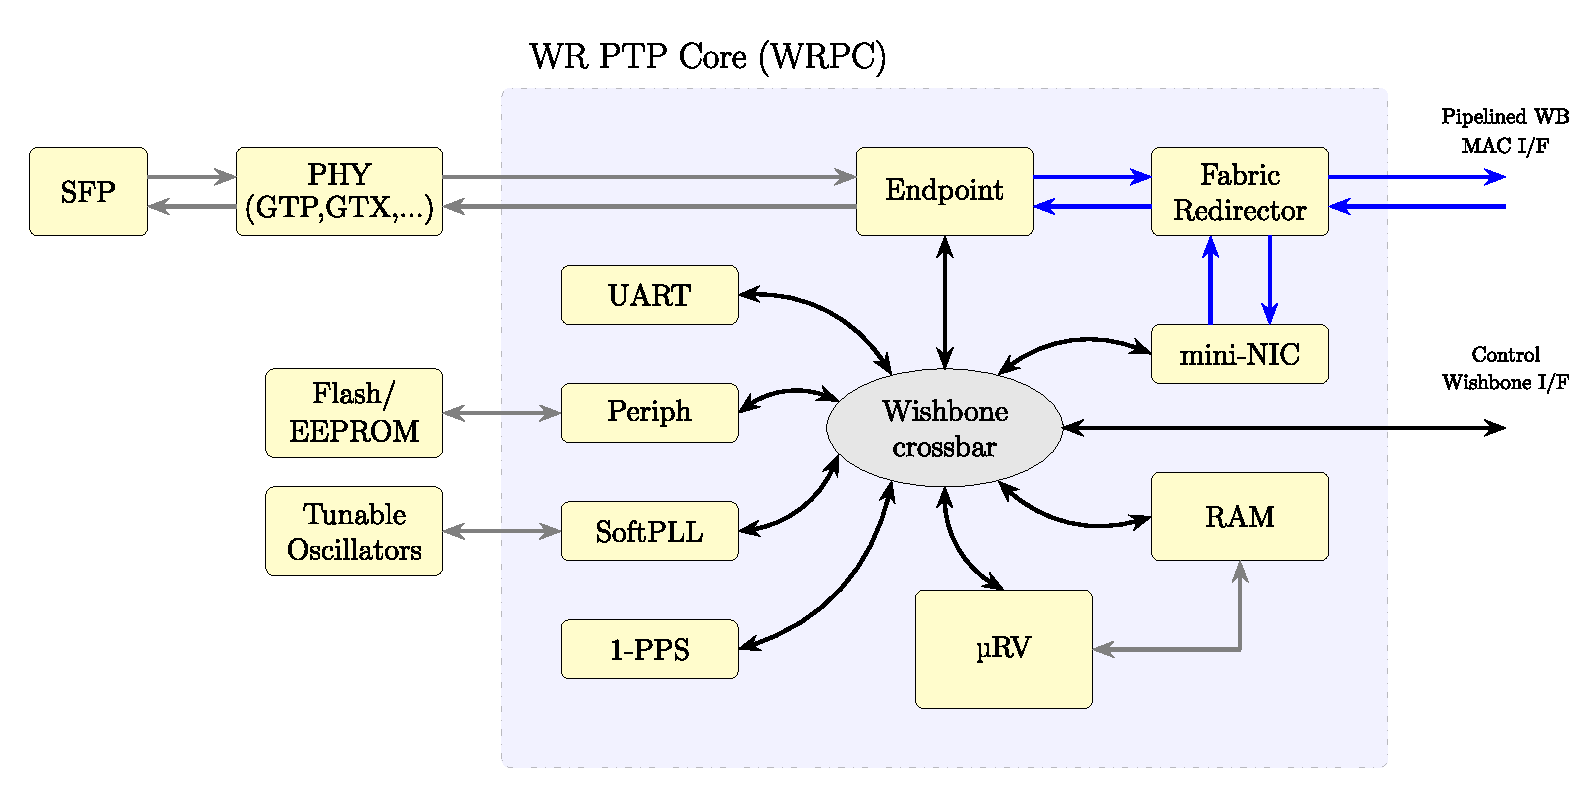
\includegraphics[width=15cm]{figures/WRPC.pdf}
    \caption{WR PTP (Precision Time Protocol) Core (WRPC).}
    \label{fig:WRPC}
\end{figure}

\noindent You can find the HDL description of the WRPC internal components in \cite{WRPC:modules}.

\subsection{\textmu RV}

The \textmu RV \cite{urv-core:ohwr} \cite{urv-core:wiki} \cite{Włostowski:2213516} (Micro RISC-V) core is a small-sized implementation of a 32-bit RISC-V core, targeted specifically at FPGAs developed by CERN. 

\begin{figure}[H]
    \centering
    
\includegraphics[width=5cm]{figures/urv_logo.png}
    \caption{\textmu RV logo.}
    \label{fig:urv}
\end{figure}

\begin{itemize}
\item Features:
    \begin{itemize}
    \item[>] Supports RV32IM instruction set. 
Division and multiply high instructions are optional and can be emulated to lower the FPGA footprint.
    \item[>] Target: FPGAs.
    \item[>] 4-stage pipeline (FDXW).
    \item[>] All instructions except taken branches/division in one clock cycle.
    \item[>] Code execution from internal memory block.
    \item[>] Wishbone bus (version B.4) for peripheral access.
    \item[>] Simple interrupt handling.
    \item[>] Verilog RTL code.
    \end{itemize}
\end{itemize}

\noindent Since \textmu RV is described in verilog and most of the WRPC component is in VHDL, it will be necessary to use a \textbf{mixed simulator} supported by VUnit.
In this context, one of the best options is \say{QuestaSim}.

\vspace{5mm}

\noindent \href{https://github.com/umarcor}{Umarcor} is planning to develop a container, hosted on our server, for this purpose. 
(DONE - Questa container, with and without VUnit, available on the lab server.)

\vspace{5mm}

\noindent \textbf{Task:} Learn how to generate a testbench using both HDLs: VHDL and Verilog.
(Initial mixed simulation test DONE - Unfortunately questa is a proprietary software and our server image cannot be distributed, so this example cannot be shown on GitHub, it is only available in our private GitLab repository.)

\subsection{WRPC Simulation}

\subsubsection{WRPC v4.2 for Spartan6 - LM32}
\label{list-wrpc}

I've successfully simulated WRPC \cite{WRPC:ohwr} in its \say{v4.2} version for \textbf{Spartan6} FPGA.

\vspace{5mm}

\noindent See \href{https://github.com/Unike267/Thesis/issues/2}{github.com/Unike267/Thesis/issues/2} to check how I have done it.

\vspace{5mm}

\noindent HDL modules that form the WRPC (\say{v4.2} for Spartan6) are:

\newpage 

\begin{dig}
\item ip\_cores
    \begin{dig}
    \item etherbone-core
        \begin{dig}
        \item hdl
            \begin{dig}
            \item eb\_master\_core (VHDL)
            \item eb\_slave\_core (VHDL)
            \item eb\_usb\_core (VHDL)
            \end{dig}
        \end{dig}
    \item general-cores
        \begin{dig}
        \item modules
            \begin{dig}
            \item common (VHDL)
            \item genrams
                \begin{dig}
                \item . (VHDL)
                \item common (VHDL)
                \item generic (VHDL)
                \item xilinx (VHDL)
                \end{dig}
            \item wishbone
                \begin{dig}
                \item . (VHDL)
                \item wb\_async\_bridge (VHDL)
                \item wb\_axi4lite\_bridge (VHDL)
                \item wb\_bus\_fanout (VHDL)
                \item wb\_clock\_crossing (VHDL)
                \item wb\_crossbar (VHDL)
                \item wb\_dma (VHDL)
                \item wb\_dpram (VHDL)
                \item wb\_gpio\_port (VHDL)
                \item wb\_i2c\_bridge (VHDL)
                \item wb\_i2c\_master (VHDL)
                \item wb\_irq (VHDL)
                \item wb\_lm32
                    \begin{dig}
                    \item generated (Verilog and VHDL)
                    \item platform/spartan6 (Verilog)
                    \item src (Verilog and VHDL)
                    \end{dig}
                \item wb\_onewire\_master (Verilog and VHDL)
                \item wb\_serial\_lcd (VHDL)
                \item wb\_simple\_pwm (VHDL)
                \item wb\_simple\_timer (VHDL)
                \item wb\_slave\_adapter (VHDL)
                \item wb\_spi (Verilog and VHDL)
                \item wb\_spi\_flash (VHDL)
                \item wb\_uart (VHDL)
                \item wb\_vic (VHDL)
                \item wbgen2 (VHDL)
                \item wbgenplus (VHDL)
                \end{dig}
            \end{dig}
        \item platform/xilinx
            \begin{dig}
            \item wb\_xil\_multiboot (VHDL)
            \item wb\_xilinx\_fpga\_loader (VHDL)
            \end{dig}
        \end{dig}
    \item gn4124-core
        \begin{dig}
        \item hdl
        \begin{dig}
            \item gn4124core   
                \begin{dig}
                \item rtl
                    \begin{dig}
                    \item . (VHDL)
                    \item spartan6 (VHDL)
                    \end{dig}  
                \end{dig}            
            \item spec
                \begin{dig}
                \item ip\_cores (VHDL)
                \end{dig}  
            \end{dig}
        \end{dig}
    \end{dig}
\item modules
    \begin{dig}
    \item fabric
        \begin{dig}
        \item . (VHDL)
        \item xwrf\_loopback (VHDL)
        \end{dig}
    \item timing (VHDL)
    \item wr\_dacs (VHDL)
    \item wr\_eca (VHDL)
    \item wr\_endpoint (VHDL)
    \item wr\_mini\_nic (VHDL)
    \item wr\_pps\_gen (VHDL)
    \item wr\_si57x\_interface (VHDL)
    \item wr\_softpll\_ng (VHDL)
    \item wr\_streamers (VHDL)
    \item wr\_tbi\_phy (VHDL)
    \item wr\_tlu (VHDL)
    \item wrc\_core (VHDL)
    \end{dig}
\item platform
    \begin{dig}
    \item xilinx
        \begin{dig}
        \item . (VHDL)
        \item wr\_gtp\_phy
            \begin{dig}
            \item . (VHDL)
            \item spartan6 (VHDL)
            \end{dig}
        \end{dig}
    \end{dig}
\end{dig}

\newpage 

\noindent HDL files for simulation are:

\begin{dig}
\item sim
    \begin{dig}
    \item endpoint\_mdio.v
    \item endpoint\_regs.v
    \item eth\_packet.svh
    \item if\_wb\_link.svh
    \item if\_wb\_master.svh
    \item if\_wb\_slave.svh
    \item if\_wishbone\_accessor.svh
    \item if\_wishbone\_types.svh
    \item lbk\_regs.v
    \item minic\_regs.vh
    \item simdrv\_defs.svh
    \item tbi\_utils.sv
    \item wb\_fabric\_defs.svh
    \item wb\_packet\_sink.svh
    \item wb\_packet\_source.svh
    \item wrc\_syscon\_regs.vh
    \item drivers:
        \begin{dig}
        \item simdrv\_minic.svh
        \item simdrv\_wr\_endpoint.svh 
        \end{dig}
    \end{dig}
\item testbench
    \begin{dig}
    \item wrc\_core
        \begin{dig}
        \item main.sv 
        \item functions.svh 
        \end{dig}
    \end{dig}
\end{dig}

\vspace{5mm}

\noindent According to this list of modules, I've generated the following block diagram shown in \ref{fig:dig}.

\vspace{5mm}

\noindent The green zone of the figure corresponds to the modules located in the \say{ip\_core} directory, the red zone to those in \say{modules}, and the blue zone to those in \say{platform}.

\begin{landscape}
\newgeometry{
	paper=a4paper, % Change to letterpaper for US letter
	inner=1cm, % Inner margin
	outer=4cm, % Outer margin
	bindingoffset=.5cm, % Binding offset
	top=12cm, % Top margin
	bottom=-5cm, % Bottom margin
	%showframe, % Uncomment to show how the type block is set on the page
}

\begin{figure}[H]
    \centering
    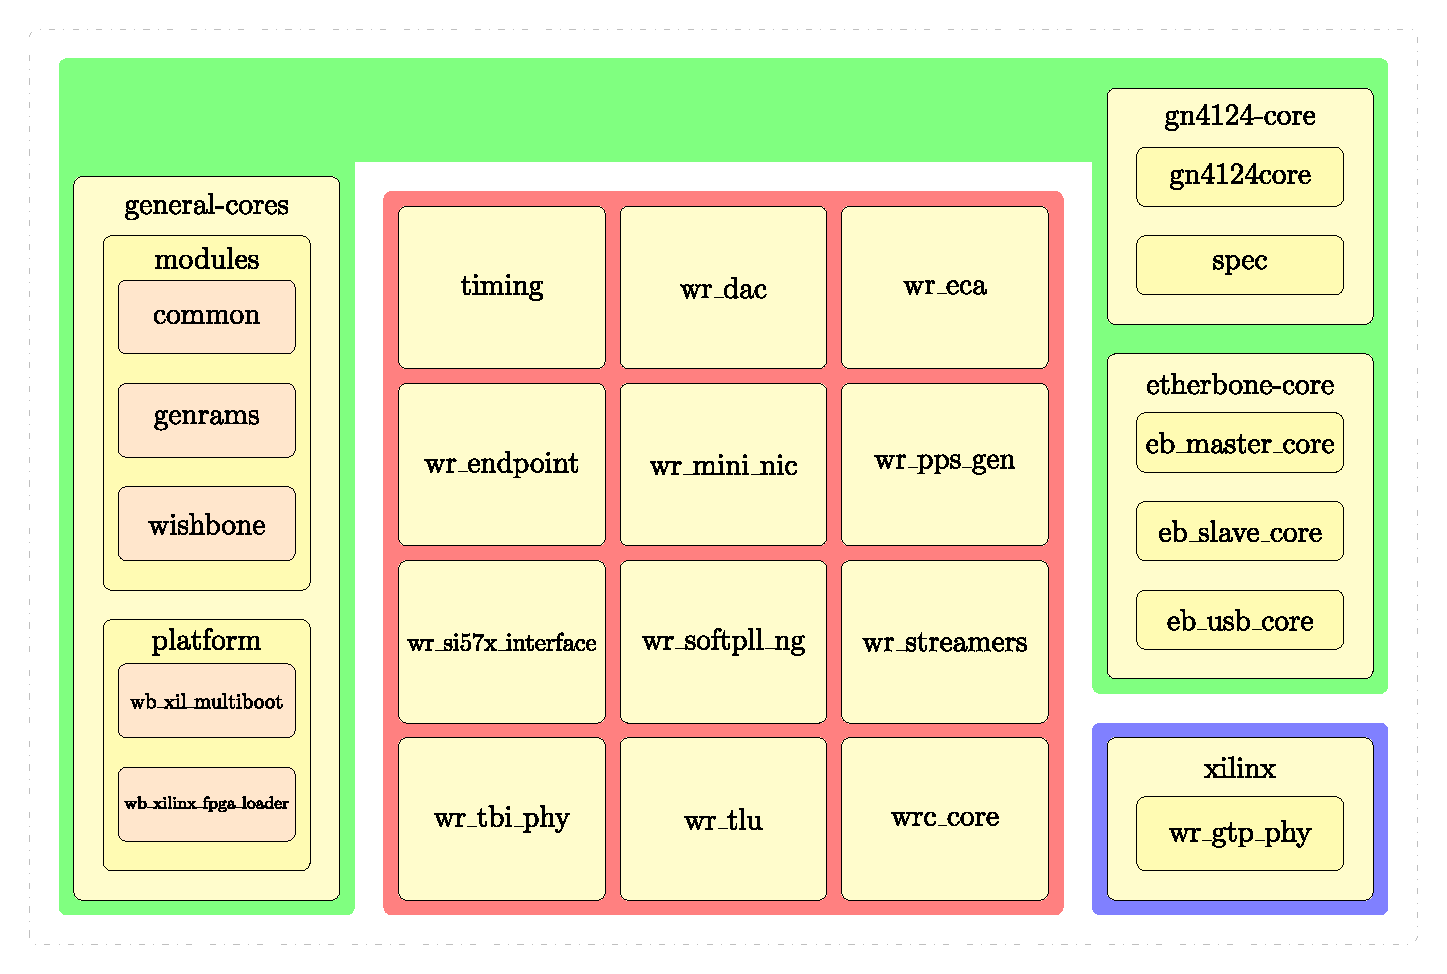
\includegraphics[width=26cm]{figures/wrpc-sources-diagram.pdf}
    \captionsetup{name=\hspace{8.5cm}Figure,format=plain,justification=centering,width=20cm}
    \caption{Block diagram of WRPC v4.2 sources for Spartan6.}
    \label{fig:dig}
\end{figure}
\restoregeometry
\end{landscape}

\noindent Taking a closer look at the \say{main.sv} testbench, I summarized the inputs and outputs of the four different modules imported into the test, which are:

\begin{itemize}
\item Clock/reset generator
\item Design Under Test: WRPC
\item Endpoint
\item Loopback
\end{itemize}

\noindent The following list presents them:

\begin{dig}
\item tbi\_clock\_rst\_gen/clkgen:
    \begin{dig}
    \item OUTPUTS:
        \begin{dig}
        \item .clk\_ref\_o                    (clk\_ref)
        \item .clk\_sys\_o                    (clk\_sys)
        \item .phy\_rbclk\_o                  (phy\_rbclk)
        \item .rst\_n\_o                      (rst\_n)
        \end{dig}
    \end{dig}
\item wr\_core/DUT (WR PTP CORE):
    \begin{dig}
    \item INPUTS:
        \begin{dig}
        \item .clk\_sys\_i                    (clk\_sys)
        \item .clk\_dmtd\_i                   (clk\_ref)
        \item .clk\_ref\_i                    (clk\_ref)
        \item .rst\_n\_i                      (rst\_n)
        \item UART:
            \begin{dig}
            \item .uart\_rxd\_i                   (1'b0)
            \end{dig}
        \item I2C:
            \begin{dig}
            \item .scl\_i                      (scl\_loop)
            \item .sda\_i                      (sda\_loop)
            \end{dig}
        \item .btn1\_i                     (1'b0)
        \item .btn2\_i                     (1'b0)
        \item Connected to wrf\_loopback:
            \begin{dig}
            \item .ext\_snk\_adr\_i              (wrc\_snk\_adr)
            \item .ext\_snk\_dat\_i              (wrc\_snk\_dat)
            \item .ext\_snk\_sel\_i              (wrc\_snk\_sel)
            \item .ext\_snk\_cyc\_i              (wrc\_snk\_cyc)
            \item .ext\_snk\_we\_i               (1'b1)
            \item .ext\_snk\_stb\_i              (wrc\_snk\_stb)
            \item 
            \item .ext\_src\_ack\_i              (wrc\_src\_ack)
            \item .ext\_src\_err\_i              (wrc\_src\_err)
            \item .ext\_src\_stall\_i            (wrc\_src\_stall)
            \end{dig}
        \item WISHBONE:
            \begin{dig}
            \item .wb\_adr\_i                   (WB\_wrc.master.adr[31:0])
            \item .wb\_dat\_i                   (WB\_wrc.master.dat\_o)
            \item .wb\_sel\_i                   (4'b1111)
            \item .wb\_we\_i                    (WB\_wrc.master.we)
            \item .wb\_cyc\_i                   (WB\_wrc.master.cyc)
            \item .wb\_stb\_i                   (WB\_wrc.master.stb)
            \end{dig}
        \item PHY:
            \begin{dig}
            \item .phy\_ref\_clk\_i              (clk\_ref)
            \item .phy\_tx\_disparity\_i         (phy\_tx\_disparity)
            \item .phy\_tx\_enc\_err\_i           (phy\_tx\_enc\_err)
            \item .phy\_rx\_rbclk\_i             (clk\_ref)
            \item .phy\_rx\_data\_i              (phy\_rx\_data)
            \item .phy\_rx\_k\_i                 (phy\_rx\_k)
            \item .phy\_rx\_enc\_err\_i           (phy\_rx\_enc\_err)
            \item .phy\_rx\_bitslide\_i          (phy\_rx\_bitslide)
            \end{dig}
        \end{dig}
    \item OUTPUTS:
        \begin{dig}
        \item .pps\_p\_o                    ()
        \item .dac\_hpll\_load\_p1\_o         ()
        \item .dac\_hpll\_data\_o            ()
        \item .dac\_dpll\_load\_p1\_o         ()
        \item .dac\_dpll\_data\_o            ()
        \item UART:
            \begin{dig}
            \item .uart\_txd\_o                 ()
            \end{dig}
        \item I2C:
            \begin{dig}
            \item .scl\_o                      (scl\_loop)
            \item .sda\_o                      (sda\_loop)
            \end{dig}
        \item .led\_link\_o                 (link\_up)
        \item connected to wrf\_loopback
            \begin{dig}
            \item .ext\_snk\_ack\_o              (wrc\_snk\_ack)
            \item .ext\_snk\_err\_o              (wrc\_snk\_err)
            \item .ext\_snk\_stall\_o            (wrc\_snk\_stall)
            \item 
            \item .ext\_src\_adr\_o              (wrc\_src\_adr)
            \item .ext\_src\_dat\_o              (wrc\_src\_dat)
            \item .ext\_src\_sel\_o              (wrc\_src\_sel)
            \item .ext\_src\_cyc\_o              (wrc\_src\_cyc)
            \item .ext\_src\_stb\_o              (wrc\_src\_stb)
            \item .ext\_src\_we\_o               ()
            \end{dig}
        \item WISHBONE:
            \begin{dig}
            \item .wb\_dat\_o                   (WB\_wrc.master.dat\_i)
            \item .wb\_ack\_o                   (WB\_wrc.master.ack)
            \item .wb\_stall\_o                 (WB\_wrc.master.stall)
            \end{dig}
        \item PHY:
            \begin{dig}
            \item .phy\_tx\_data\_o              (phy\_tx\_data)
            \item .phy\_tx\_k\_o                 (phy\_tx\_k)
            \item .phy\_rst\_o                  (phy\_rst)
            \item .phy\_loopen\_o               (phy\_lo)
            \end{dig}
        \end{dig}
    \end{dig}
\item wr\_endpoint/EP (ENDPOINT):
    \begin{dig}
    \item INPUTS:
        \begin{dig}
        \item .clk\_ref\_i                  (clk\_ref)
        \item .clk\_sys\_i                  (clk\_sys)
        \item .clk\_dmtd\_i                 (clk\_ref)
        \item .rst\_sys\_n\_i                (rst\_n)
        \item .rst\_ref\_n\_i                (rst\_n)
        \item .rst\_dmtd\_n\_i               (rst\_n)
        \item .rst\_txclk\_n\_i              (rst\_n)
        \item .rst\_rxclk\_n\_i              (rst\_n)
        \item .pps\_csync\_p1\_i             (1'b0)
        \item PHY:
            \begin{dig}
            \item .phy\_sfp\_tx\_fault\_i         (1'b0)
            \item .phy\_sfp\_los\_i              (1'b0)
            \item .phy\_rdy\_i                  (1'b1)
            \item .phy\_ref\_clk\_i              (clk\_ref)
            \item .phy\_tx\_disparity\_i         (phy\_tx\_disparity)
            \item .phy\_tx\_enc\_err\_i           (phy\_tx\_enc\_err)
            \item .phy\_rx\_data\_i              (phy\_tx\_data)
            \item .phy\_rx\_clk\_i               (clk\_ref)
            \item .phy\_rx\_k\_i                 (phy\_tx\_k)
            \item .phy\_rx\_enc\_err\_i           (phy\_rx\_enc\_err)
            \item .phy\_rx\_bitslide\_i          (phy\_rx\_bitslide)
            \end{dig}
        \item Connected to simulation:
            \begin{dig}
            \item .src\_stall\_i                (WB\_ep\_snk.slave.stall)
            \item .src\_ack\_i                  (WB\_ep\_snk.slave.ack)
            \item .src\_err\_i                  (1'b0)
            \item 
            \item .snk\_dat\_i                  (WB\_ep\_src.master.dat\_o)
            \item .snk\_adr\_i                  (WB\_ep\_src.master.adr)
            \item .snk\_sel\_i                  (WB\_ep\_src.master.sel)
            \item .snk\_cyc\_i                  (WB\_ep\_src.master.cyc)
            \item .snk\_stb\_i                  (WB\_ep\_src.master.stb)
            \item .snk\_we\_i                   (WB\_ep\_src.master.we)
            \end{dig}
        \item WISHBONE:
            \begin{dig}
            \item .wb\_cyc\_i                   (WB\_ep.master.cyc)
            \item .wb\_stb\_i                   (WB\_ep.master.stb)
            \item .wb\_we\_i                    (WB\_ep.master.we)
            \item .wb\_sel\_i                   (WB\_ep.master.sel)
            \item .wb\_adr\_i                   (WB\_ep.master.adr[7:0])
            \item .wb\_dat\_i                   (WB\_ep.master.dat\_o)
            \end{dig}
        \end{dig}
    \item OUTPUTS:
        \begin{dig}
        \item PHY:
            \begin{dig}
            \item .phy\_tx\_data\_o              (phy\_rx\_data)
            \item .phy\_tx\_k\_o                 (phy\_rx\_k)
            \end{dig}
        \item Connected to simulation:
            \begin{dig}
            \item .src\_dat\_o                  (WB\_ep\_snk.slave.dat\_i)
            \item .src\_adr\_o                  (WB\_ep\_snk.slave.adr)
            \item .src\_sel\_o                  (WB\_ep\_snk.slave.sel)
            \item .src\_cyc\_o                  (WB\_ep\_snk.slave.cyc)
            \item .src\_stb\_o                  (WB\_ep\_snk.slave.stb)
            \item .src\_we\_o                   (WB\_ep\_snk.slave.we)
            \item 
            \item .snk\_stall\_o                (WB\_ep\_src.master.stall)
            \item .snk\_ack\_o                  (WB\_ep\_src.master.ack)
            \item .snk\_err\_o                  (WB\_ep\_src.master.err)
            \end{dig}
        \item WISHBONE:
            \begin{dig}
            \item .wb\_dat\_o                   (WB\_ep.master.dat\_i)
            \item .wb\_ack\_o                   (WB\_ep.master.ack)
            \item .wb\_stall\_o                 (WB\_ep.master.stall));
            \end{dig}
        \end{dig}
    \end{dig}
\item wrf\_loopback/WRF\_LBK (LOOPBACK): 
    \begin{dig}
    \item INPUTS:
        \begin{dig}
        \item .clk\_sys\_i                  (clk\_sys)
        \item .rst\_n\_i                    (rst\_n)
        \item Connected to wr\_core:
            \begin{dig}
            \item .snk\_cyc\_i                  (wrc\_src\_cyc)
            \item .snk\_stb\_i                  (wrc\_src\_stb)
            \item .snk\_we\_i                   (1'b1)
            \item .snk\_sel\_i                  (wrc\_src\_sel)
            \item .snk\_adr\_i                  (wrc\_src\_adr)
            \item .snk\_dat\_i                  (wrc\_src\_dat)
            \item 
            \item .src\_ack\_i                  (wrc\_snk\_ack)
            \item .src\_stall\_i                (wrc\_snk\_stall)
            \end{dig}
        \item WISHBONE:
            \begin{dig}
            \item .wb\_cyc\_i                   (WB\_lbk.master.cyc)
            \item .wb\_stb\_i                   (WB\_lbk.master.stb)
            \item .wb\_we\_i                    (WB\_lbk.master.we)
            \item .wb\_sel\_i                   (4'b1111)
            \item .wb\_adr\_i                   (WB\_lbk.master.adr)
            \item .wb\_dat\_i                   (WB\_lbk.master.dat\_o)
            \end{dig}
        \end{dig}
    \item OUTPUTS:
        \begin{dig}
        \item Connected to wr\_core:
            \begin{dig}
            \item .snk\_ack\_o                  (wrc\_src\_ack)
            \item .snk\_stall\_o                (wrc\_src\_stall)
            \item 
            \item .src\_cyc\_o                  (wrc\_snk\_cyc)
            \item .src\_stb\_o                  (wrc\_snk\_stb)
            \item .src\_we\_o                   ()
            \item .src\_sel\_o                  (wrc\_snk\_sel)
            \item .src\_adr\_o                  (wrc\_snk\_adr)
            \item .src\_dat\_o                  (wrc\_snk\_dat)
            \end{dig}
        \item WISHBONE:
            \begin{dig}
            \item .wb\_dat\_o                   (WB\_lbk.master.dat\_i)
            \item .wb\_ack\_o                   (WB\_lbk.master.ack)
            \end{dig}
        \end{dig}
    \end{dig}
\end{dig}

\newpage 

\subsubsection{WRPC v4.2 for Spartan6 - Test bench flow}

\noindent The testbench I used to simulate the WRPC is located in \href{https://gitlab.com/ohwr/project/wr-cores/-/tree/master/testbench/wrc_core}{testbench/wrc\_core}, and the following image summarizes its behavior:

\begin{figure}[H]
\centering
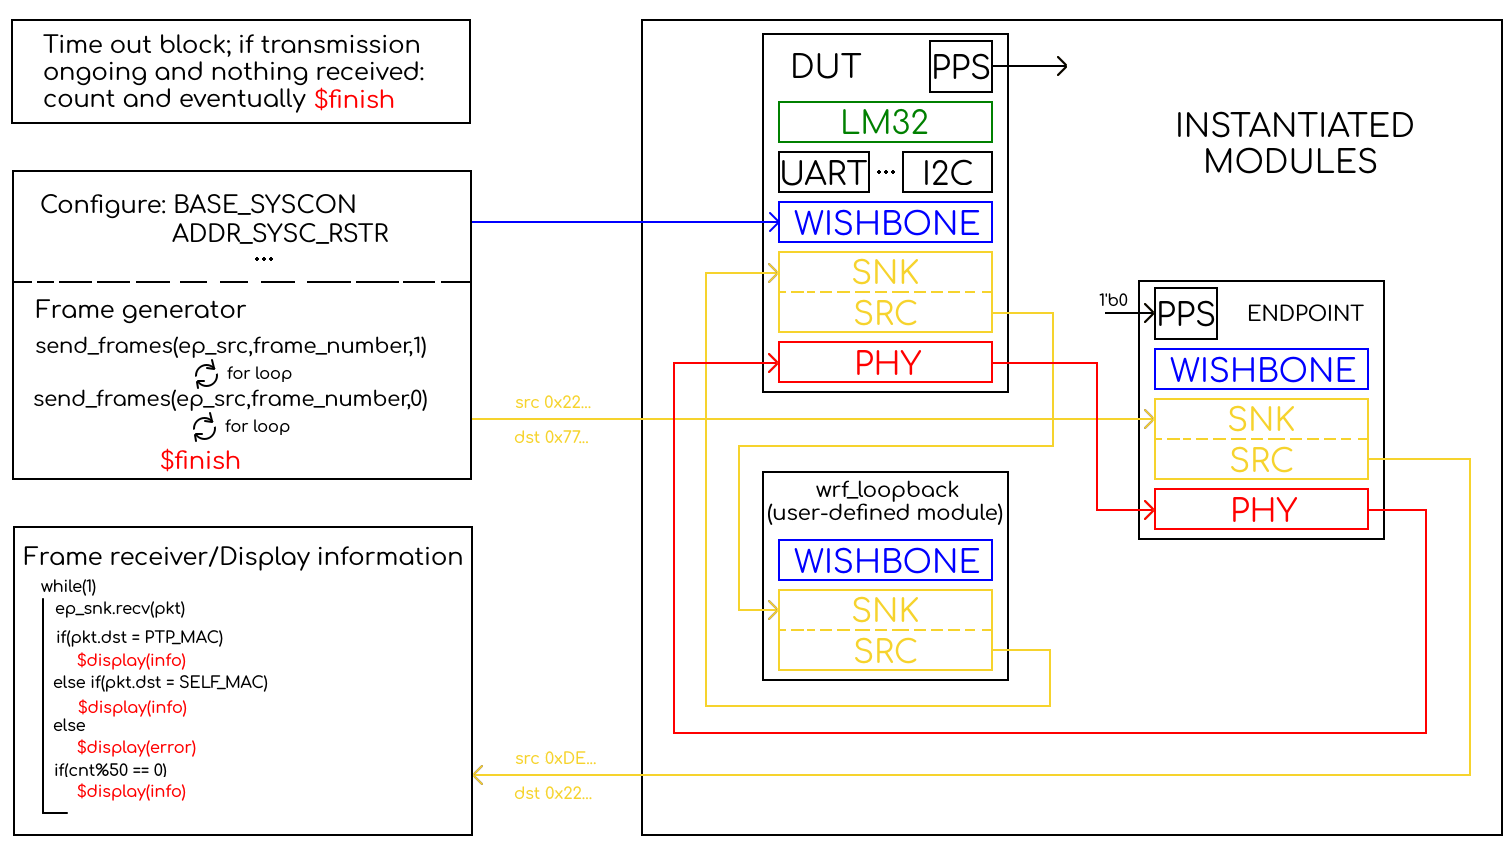
\includegraphics[width=14cm]{figures/tb_scheme.png}
\caption{Scheme of the testbench.}
\label{fig:tb-scheme}
\end{figure}

\noindent As shown on the left side of Figure \ref{fig:tb-scheme}, the testbench code is divided into three main structures:

\begin{itemize}
\item \say{Timeout mechanism}
\item \say{Configure – Frame generator}
\item \say{Frame receiver and information displayer}
\end{itemize}

\noindent The \say{Timeout mechanism} structure is the timeout block, which ends the testbench if a transmission is ongoing and no frames are received.

\vspace{5mm}

\noindent The \say{Configure – Frame generator} structure sends the configuration via the DUT’s external Wishbone interface to its internal Wishbone crossbar.
It then uses the function \say{send\_frames} (defined in the \say{functions.svh} file) to generate Ethernet frames and inject them through the ENDPOINT’s external fabric interface.
This frame generation/injection loop continues until the specified number of frames (frame\_number) is generated/sent.
After that, the process starts again, this time changing the IFG (Inter Frame Gap) from one (fixed) to zero (random).
When this second phase finishes, and if the timeout has not been triggered, the testbench ends.

\vspace{5mm}

\noindent The \say{Frame receiver and information displayer} structure receives all Ethernet frames and displays information based on the data received.
In its infinite loop, it analyzes the MAC address of each frame and determines whether it came from PTP\_MAC or SELF\_MAC.
If the MAC address does not match either, an error message is displayed.
This Ethernet frames are captured from the ENDPOINT’s external fabric interface. 
Additionally, a special status message is shown every 50 frames received.

\vspace{5mm}

\noindent The following image illustrates the flow of the testbench:

\begin{figure}[H]
\centering
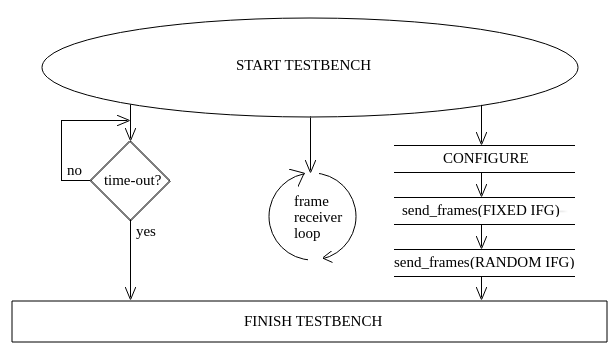
\includegraphics[width=14cm]{figures/tb_flow.png}
\caption{Test bench flow.}
\label{fig:tb-flow}
\end{figure}

\newpage 

\subsubsection{WRPC v4.2 for Spartan6 - Analysis of test bench results}

\noindent To simplify the interpretation of the testbench results, I’ve reduced the \say{number frame} constant to two.
This means there will be four frame transmissions: two with a fixed IFG and two with a random IFG.
I also modified the testbench to export the transmitted frames to a .txt file, so the transmitted data can be inspected.
The contents of this frames text file are shown in Figure \ref{fig:frame-res}.

\begin{figure}[H]
\centering
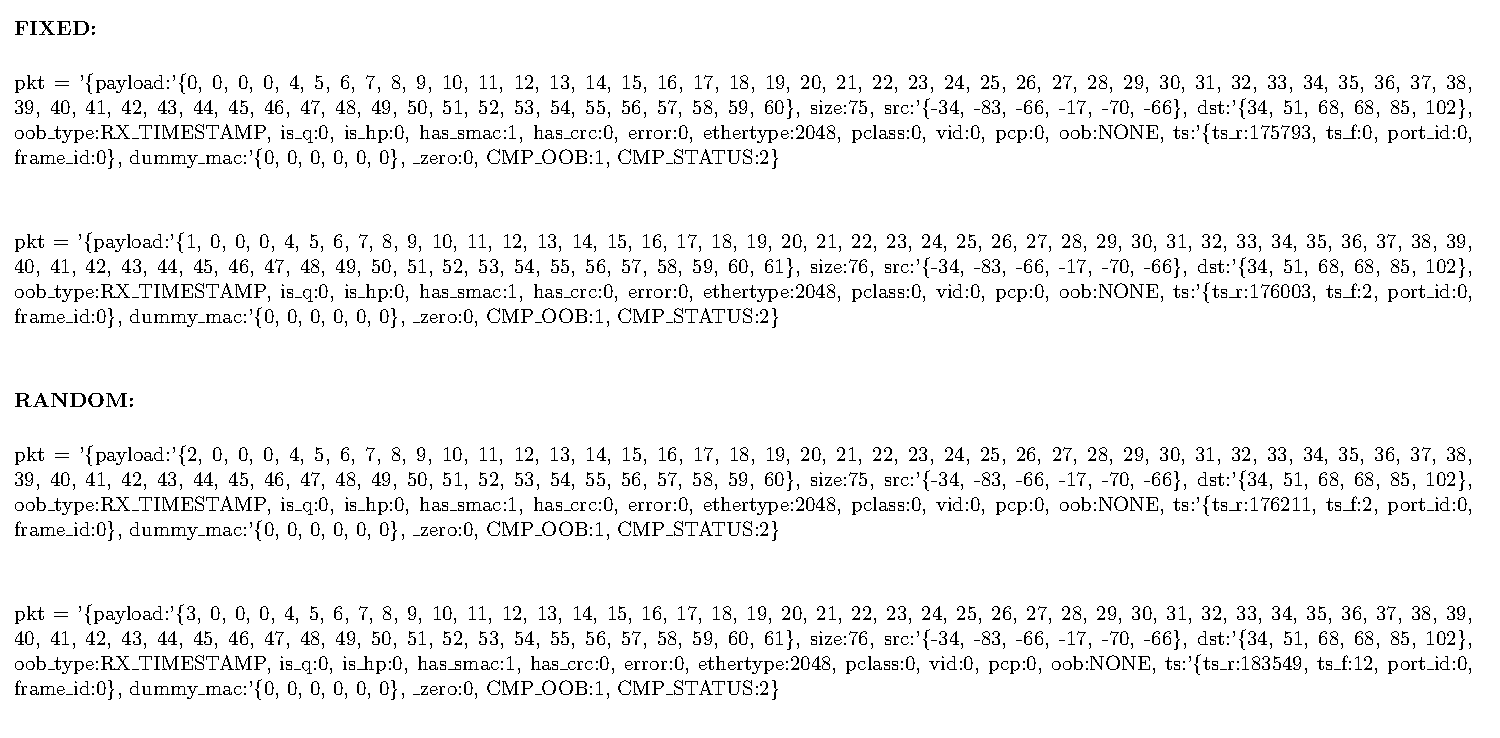
\includegraphics[width=14.5cm]{figures/frames.pdf}
\caption{Frames extraction.}
\label{fig:frame-res}
\end{figure}

\noindent Within the frame, there are many fields related to a standard Ethernet frame, but there are also some very interesting fields specific to the White Rabbit (WR) extension of PTP.
One such field is the \say{ts} field, which represents the WR timestamp.
The structure of this field is as follows:

\begin{itemize}
\item bit[27:0] ts\_r
\item bit[3:0] ts\_f
\item bit[5:0] port\_id
\item bit[15:0] frame\_id
\end{itemize}

\noindent These signals are defined in Section \textbf{8.1.6 Fabric Interface – Rx OOB Format}, of the wrpc-user manual \cite{WR-core:manual}.
Later, we will examine them in more detail when we analyze the frame.

\vspace{5mm}

\subsubsection{WRPC v4.2 for Spartan6 - CI}

\noindent This simulation has been successfully integrated into the continuous integration pipeline of the GitLab repository, see \href{https://github.com/Unike267/Thesis/issues/3}{github.com/Unike267/Thesis/ issues/3}.
Some of the most important steps that have been carried out are:

\begin{dig}
\item Compile the necessary Xilinx libraries (\say{unisim} and \say{xilinxcorelib}) using ISE as an intermediary.
\item Generate the required Makefile using the hdlmake tool \cite{hdl-make:ohwr}.
\item Run the simulation with Questasim.
\item Upload the waveform as an artifact.
\end{dig}

\vspace{1mm}

\noindent This process is illustrated graphically through the following images:

\begin{figure}[H]
\centering
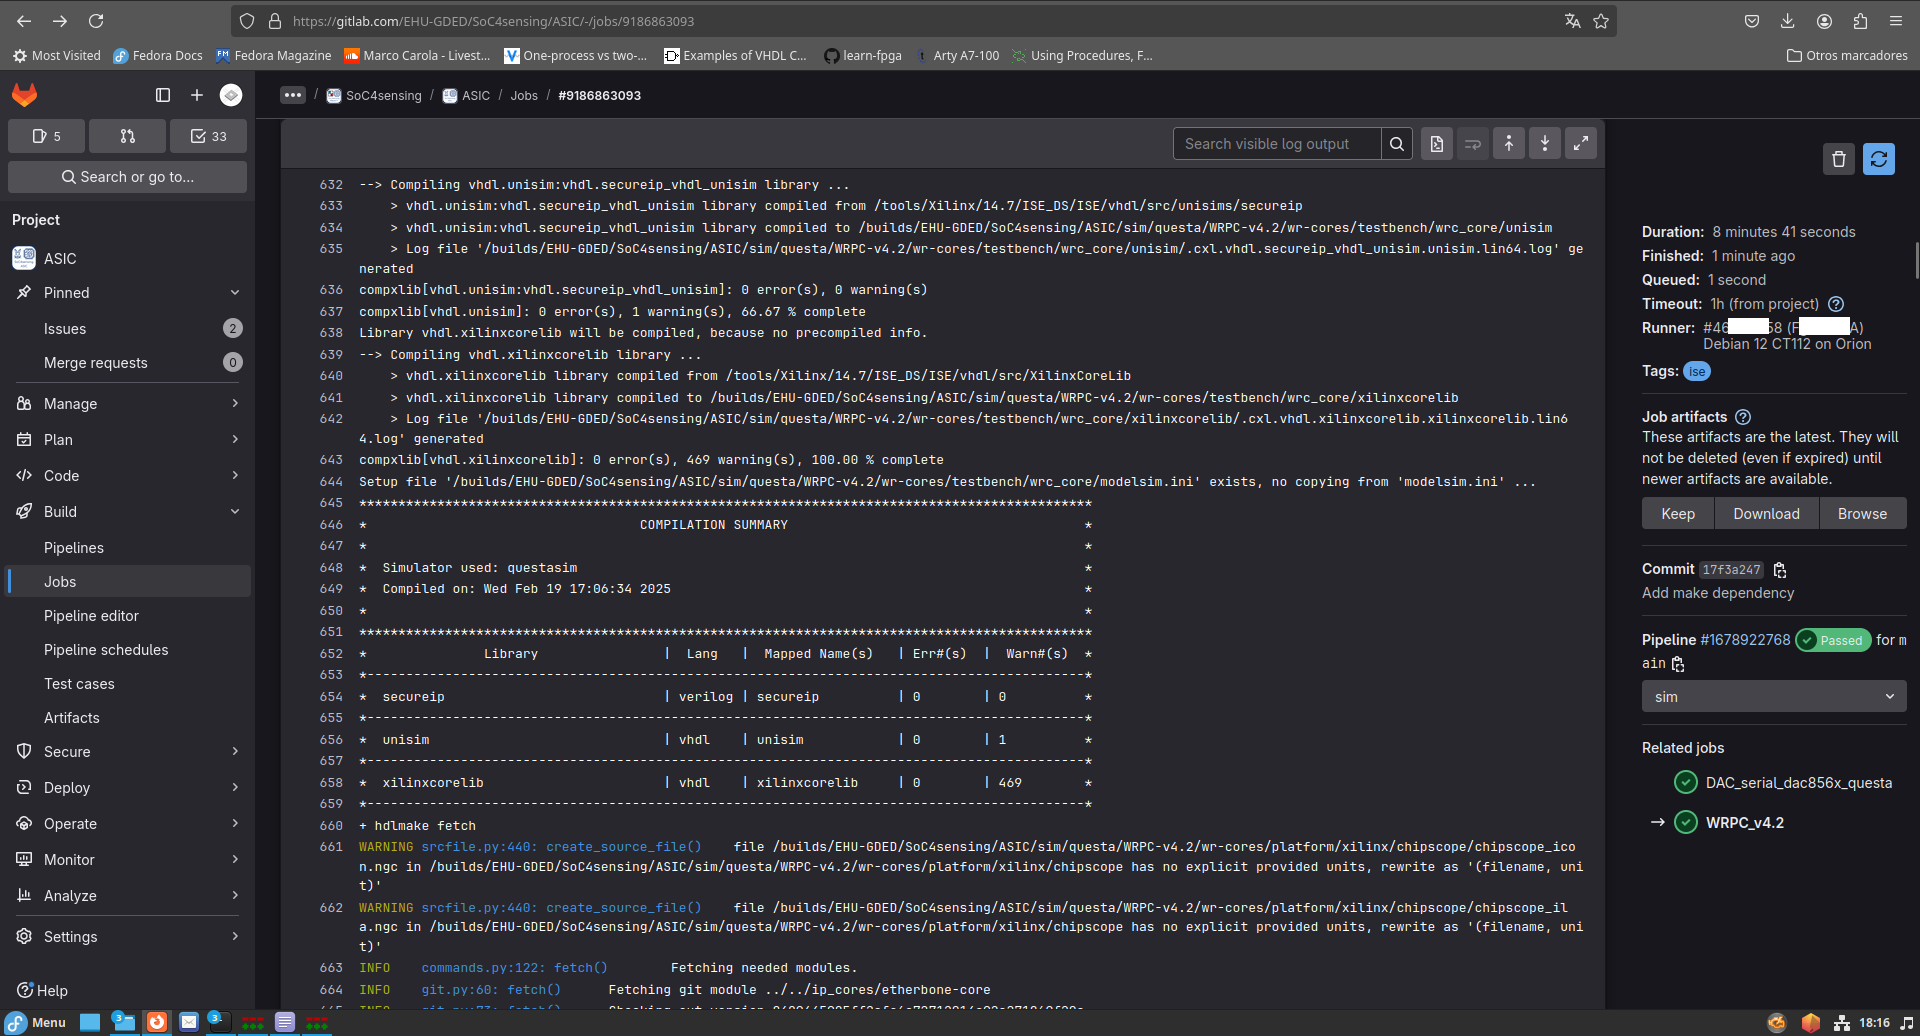
\includegraphics[width=14cm]{figures/wrpc_ci_1.png}
\caption{Compiling the Xilinx libraries and generating the Makefile.}
\label{fig:wrpc-ci-1}
\end{figure}

\begin{figure}[H]
\centering
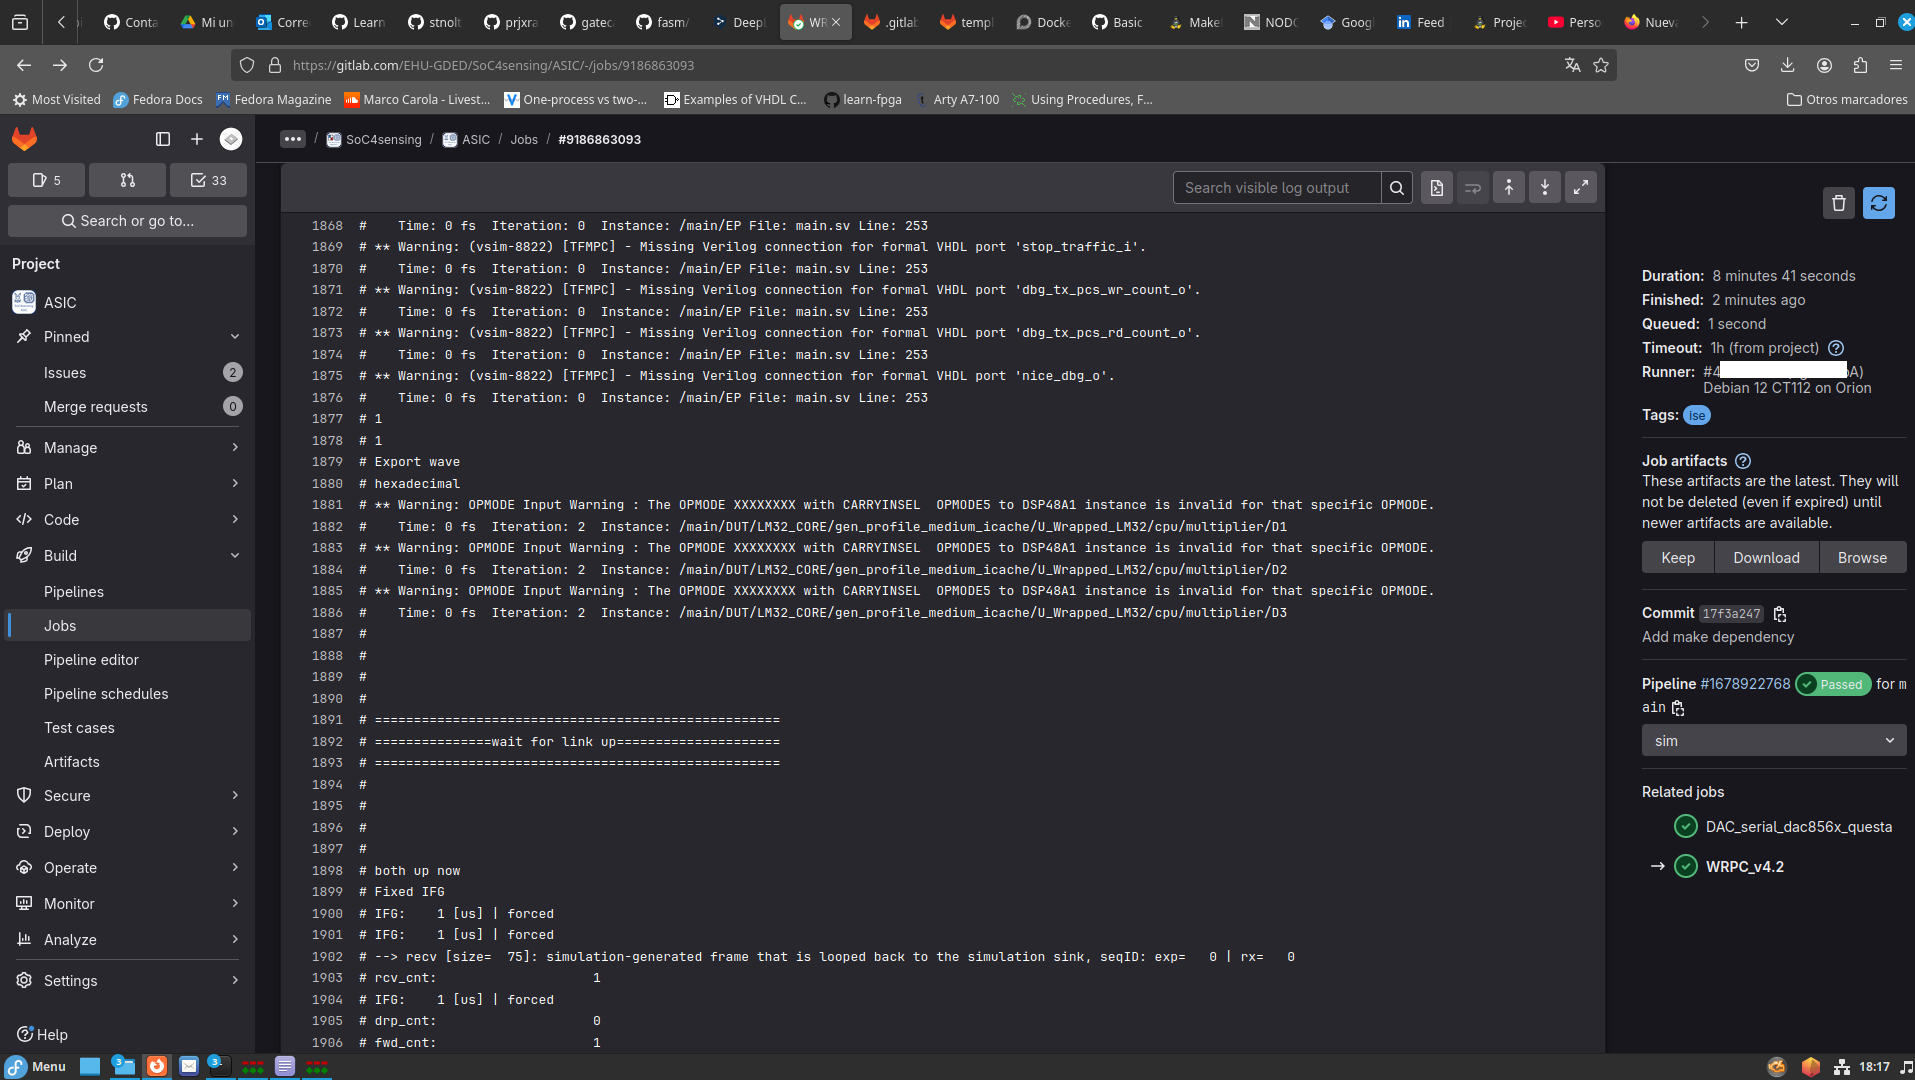
\includegraphics[width=14cm]{figures/wrpc_ci_2.png}
\caption{Running the simulation with Questasim.}
\label{fig:wrpc-ci-2}
\end{figure}

\begin{figure}[H]
\centering
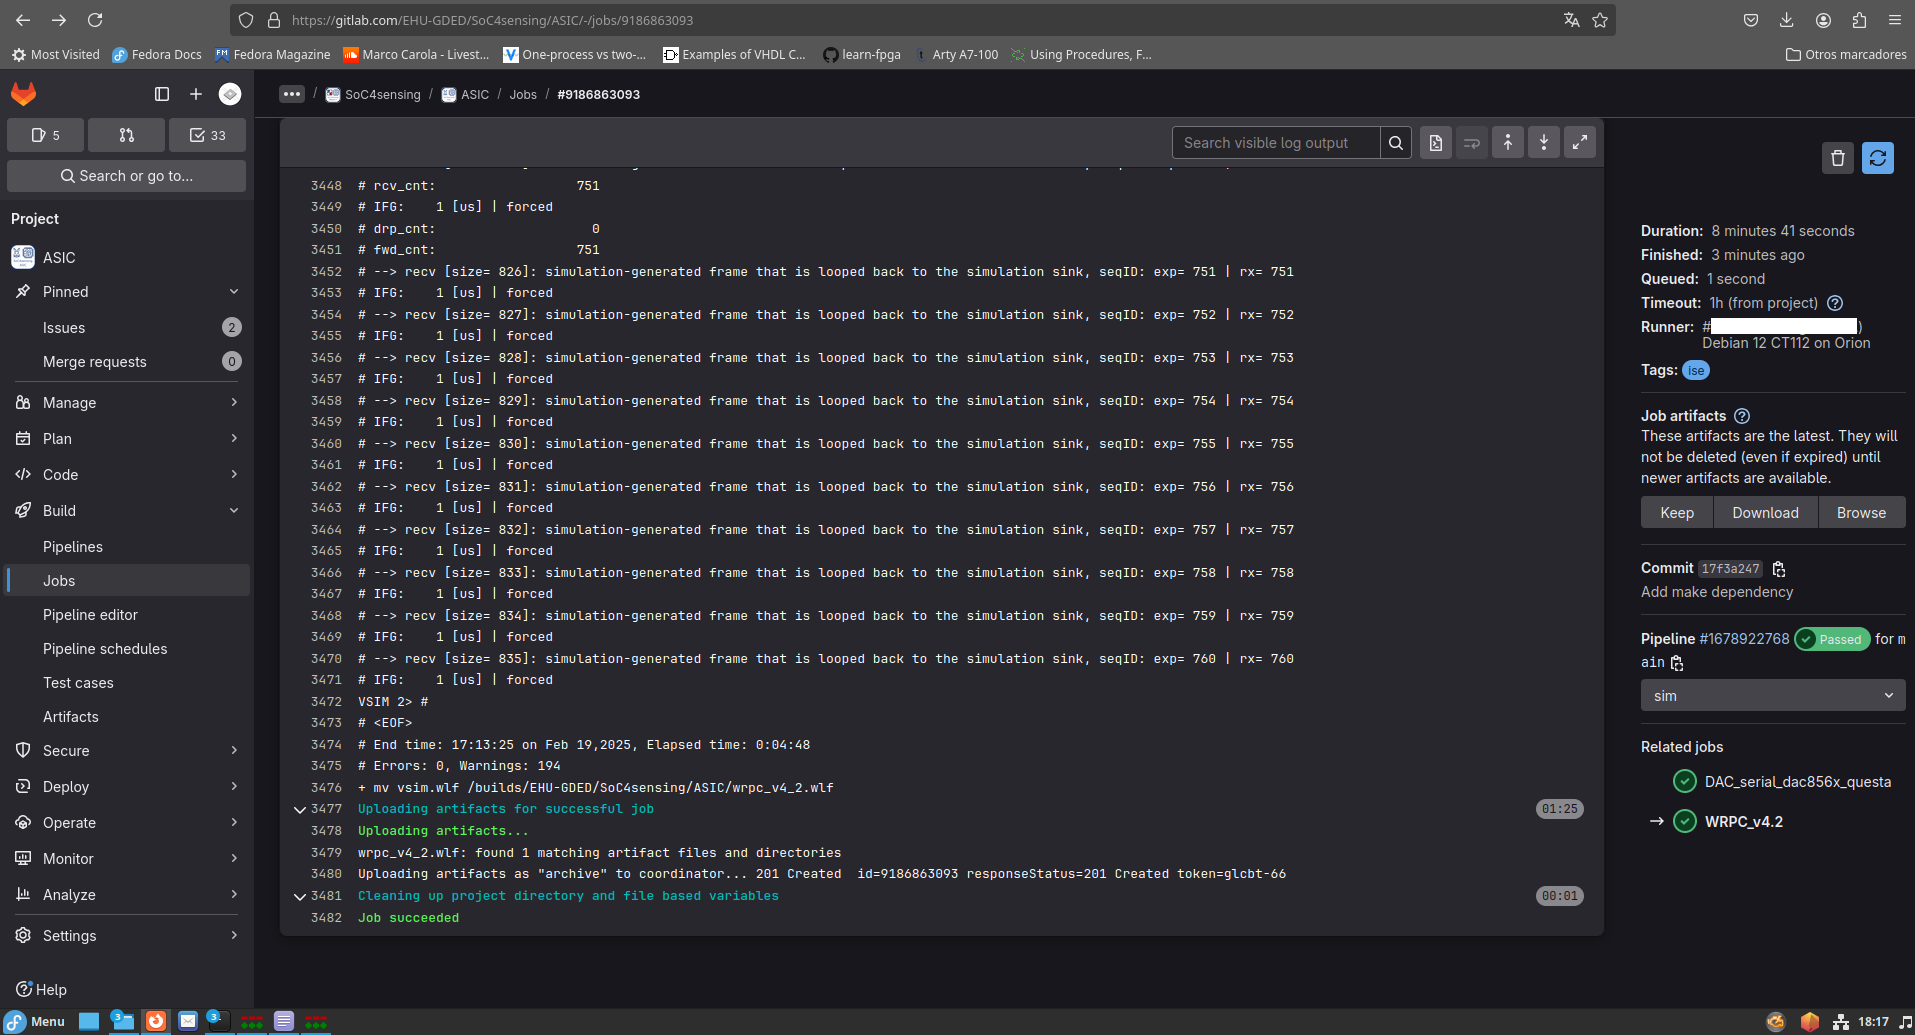
\includegraphics[width=14cm]{figures/wrpc_ci_3.png}
\caption{Uploading the waveform as an artifact.}
\label{fig:wrpc-ci-3}
\end{figure}

\subsubsection{DAC: serial\_dac856x}

\noindent As a proof of concept for performing simulation in continuous integration using free/libre tools, the \say{serial\_dac856x} DAC has been simulated.

\vspace{5mm}

\noindent This simulation was carried out using the VUnit \cite{gh:vunit} framework and the GHDL \cite{gh:ghdl} simulator.

\vspace{5mm}

\noindent Since there is no free/libre mixed-language simulator available, generating a complete WRPC simulation is not possible in the GitHub-hosted repository. However, this limitation does not apply to the GitLab repository, where we have access to a private container with Questasim and VUnit.

\vspace{5mm}

\noindent This restriction exists because several WRPC module sources are written in Verilog, see \ref{list-wrpc}.

\vspace{5mm}

\noindent The simulation results, including both the waveform and the \say{CSV} file containing the verbose output, are uploaded as artifacts and attached to the release assets, see \href{https://github.com/Unike267/Thesis/releases}{github.com/Unike267/Thesis/releases}.
